
\section{Current results Batch RL HalfCheetah}
We use one of the D4RL datasets.
Specifically \textit{halfcheetah-medium-v0}, which uses 1M samples from a policy trained
to approximately 1/3 the performance of the expert.

We introduce stochasticity in the original cost function in a way that 
makes the environment stochastic enough to have a meaningful assessment of risk in terms of 
tail performance.
A reward of -100 is given wp 0.05, if the velocity of the cheetah is greater than 4.
We train using the distributional critic and a policy that consists of a variational autoencoder
to sample from the dataset distribution and then a second perturbing network that shifts the
action towards maximizing the sampled CVaR.
The perturbation is up to 0.5 (paper originally 0.05).

\begin{figure}[ht]
        \centering
        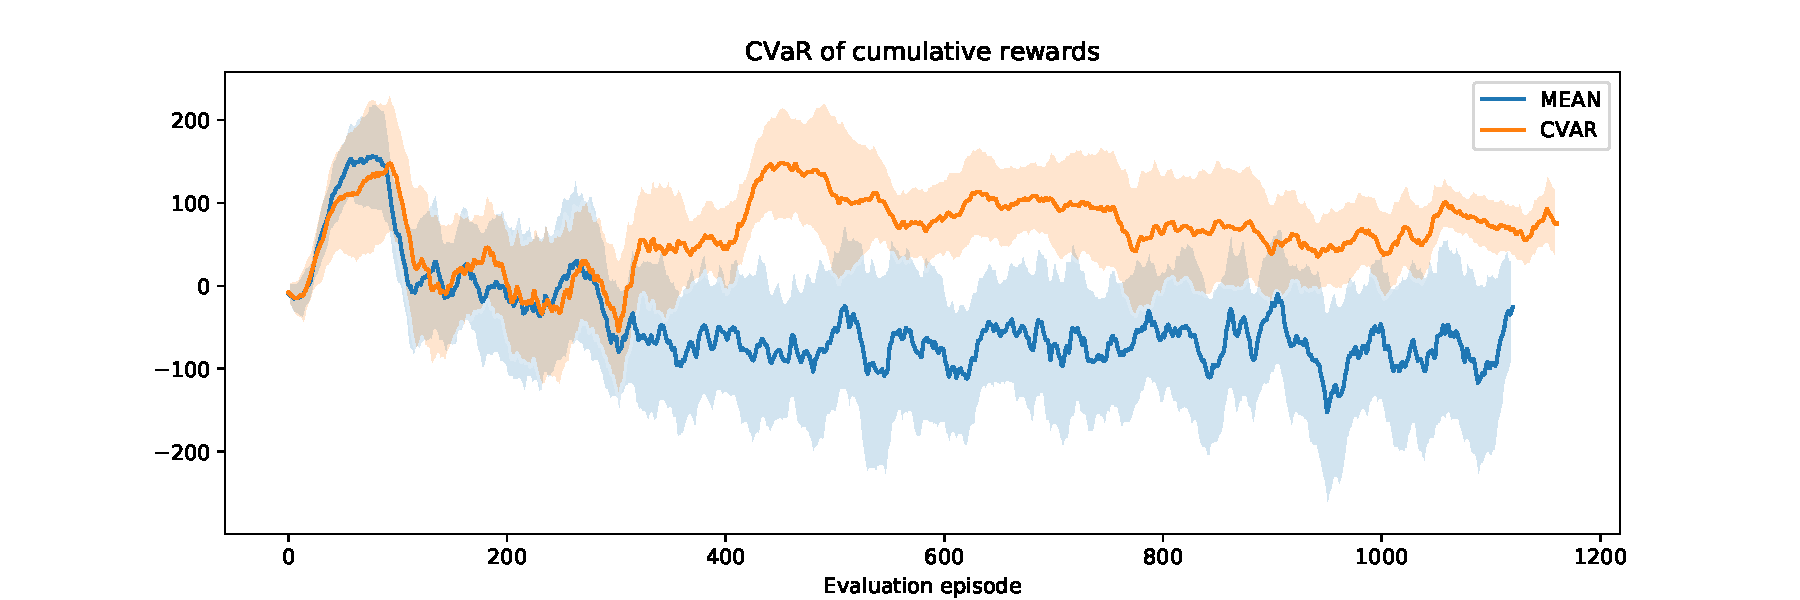
\includegraphics[width=0.8\textwidth]{images/Cheetah_offpolicy_medium/cvar_train_withstds.pdf}
        \caption{Evolution during training of CVaR ($\alpha=0.1)$ of the cumulative rewards
        over 5 evaluation episodes}
        \label{cvar_cheetah}
    
\end{figure}

\begin{figure}[ht]
    \centering
    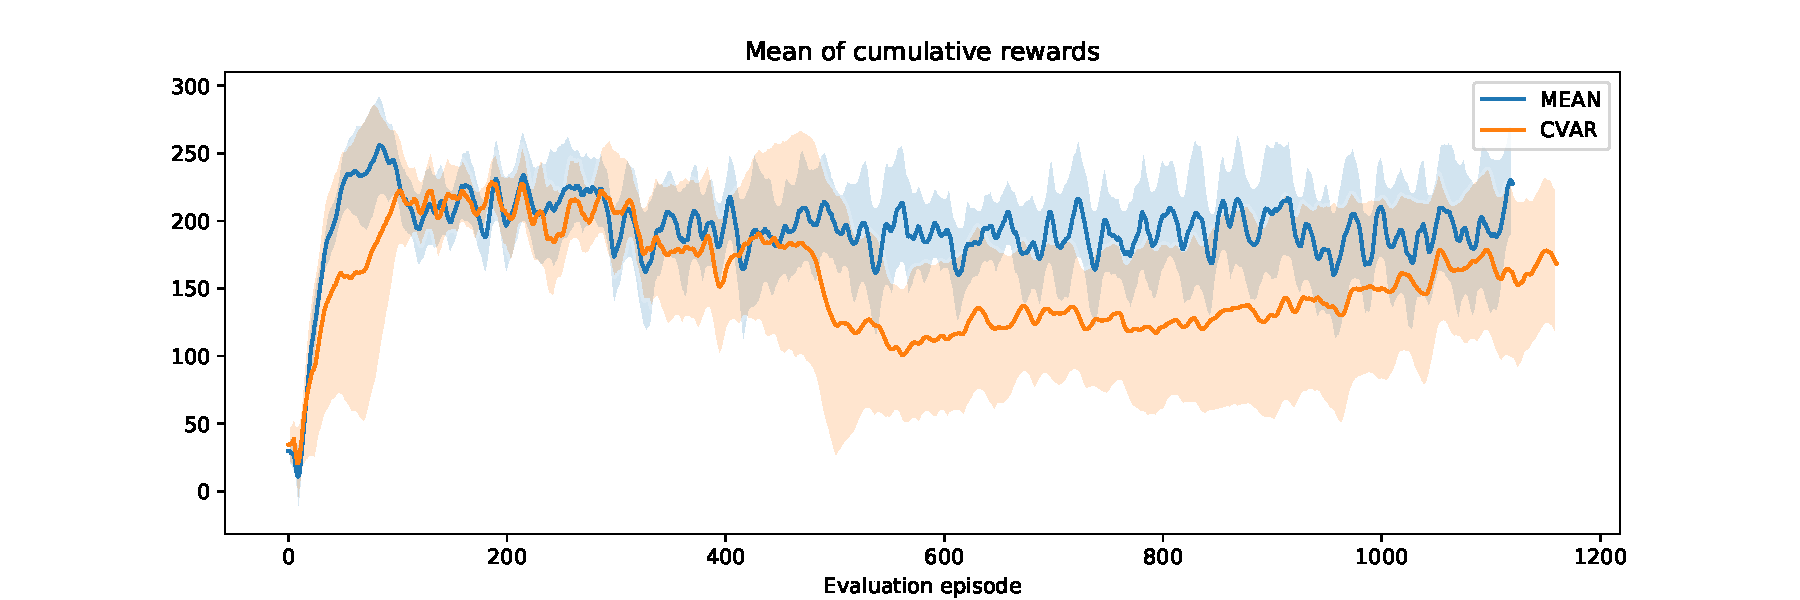
\includegraphics[width=0.8\textwidth]{images/Cheetah_offpolicy_medium/mean_train_withstds.pdf}
    \caption{Evolution during training of mean of the cumulative rewards over 5 evaluation episodes}
    \label{mean_cheetah}

\end{figure}



\begin{figure}[ht]
    \centering
    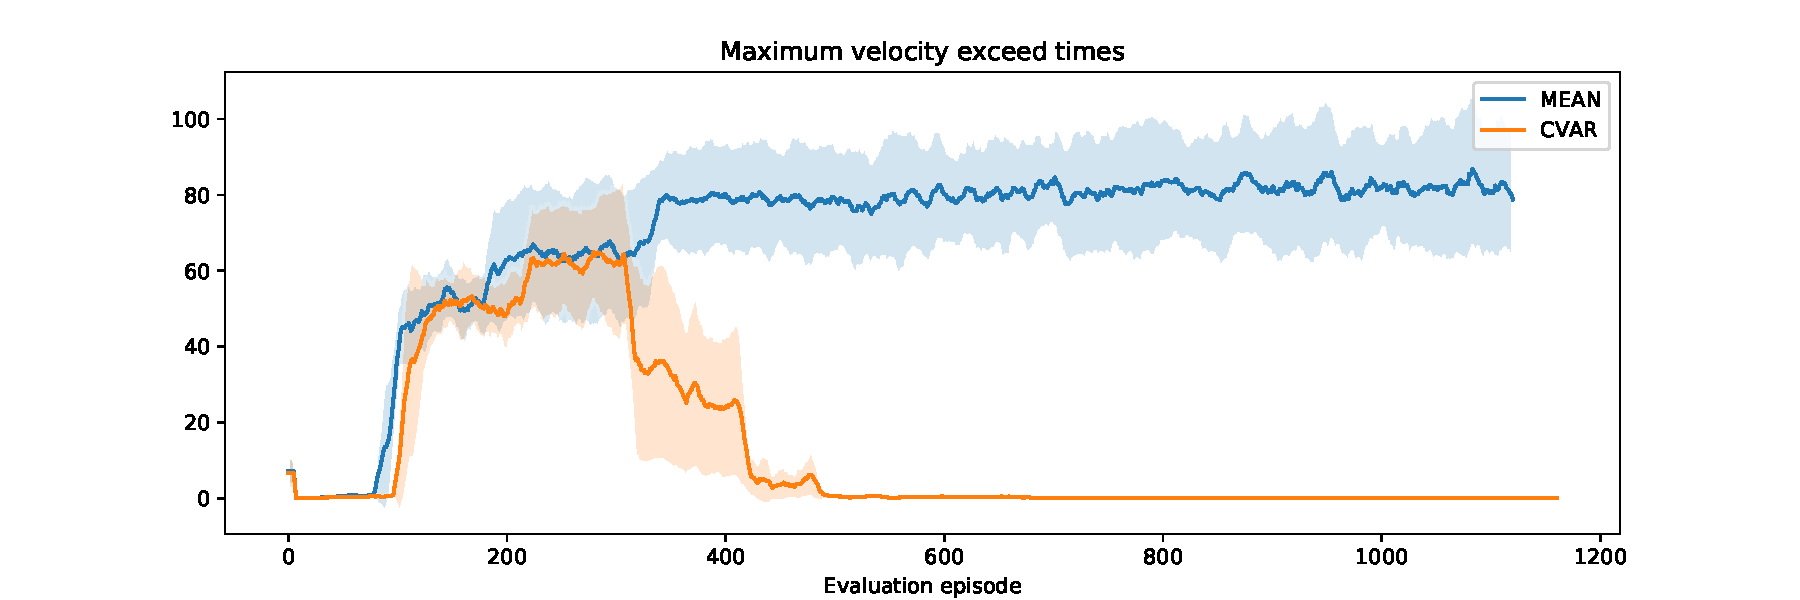
\includegraphics[width=0.8\textwidth]{images/Cheetah_offpolicy_medium/times_exceedvel_withstds.pdf}
    \caption{Evolution during training of mean of times of maximum velocity exceed over 5 evaluation episodes}
    \label{vel_exceed_cheetah}

\end{figure}

\begin{figure}[ht]
    \centering
    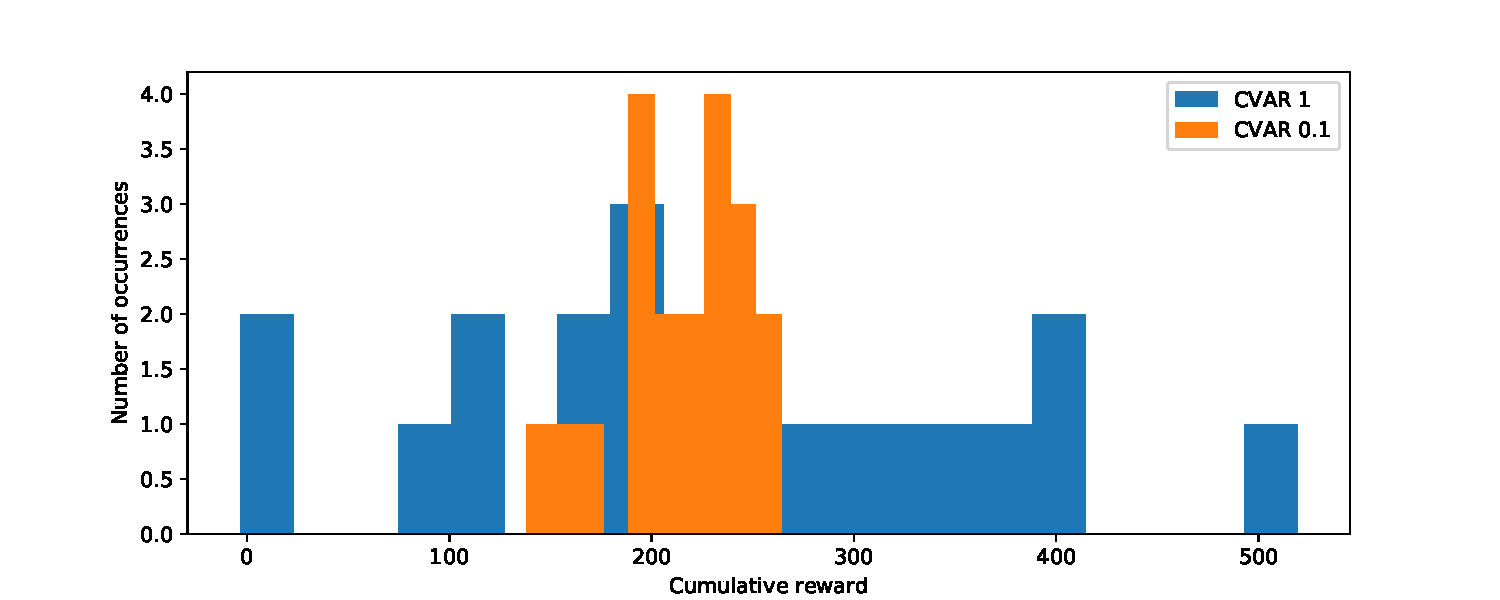
\includegraphics[width=0.8\textwidth]{images/Cheetah_offpolicy_medium/hist_evaluation_numevalsteps200.pdf}
    \caption{Histogram of cumulative rewards during 200 time steps using the trained final policies}
    \label{hist_cum_rewards200steps_cheetah}

\end{figure}